\chapter{Породжені класи множин}
\label{sec-2}

\section{Означення і елементарні властивості породжених класів множин}

Спочатку розглянемо означення породжених класів множин.

\begin{definition}
\label{def-1-7}
Нехай $\HH\subset2^X$ є непорожнім класом множин.
Клас
\begin{equation}
\label{1.4}
k(\HH)=\bigcap_{\substack{\K_\alpha\supset \HH\\ \K_\alpha\text{ є кільцем}}} \K_\alpha
\end{equation}
називається \emph{кільцем, породженим класом $\HH$}; клас
\begin{equation}
\label{1.4-1}
a(\HH)=\bigcap_{\substack{\mathcal A_\alpha\supset \HH\\ \mathcal A_\alpha\text{ є алгеброю}}} \mathcal A_\alpha
\end{equation}
називається \emph{алгеброю, породженою класом $\HH$}; клас
\begin{equation}
\label{1.4-2}
\sigma k(\HH)=\bigcap_{\substack{\K_\alpha\supset \HH\\ \K_\alpha\text{ є $\sigma$-кільцем}}} \K_\alpha
\end{equation}
називається \emph{$\sigma$-кільцем, породженим класом $\HH$}; клас
\begin{equation}
\label{1.4-3}
\sigma a(\HH)=\bigcap_{\substack{\mathcal A_\alpha\supset \HH\\ \mathcal A_\alpha\text{ є $\sigma$-алгеброю}}} \mathcal A_\alpha
\end{equation}
називається \emph{$\sigma$-алгеброю, породженою класом $\HH$}; клас
\begin{equation}
\label{1.4-4}
m(\HH)=\bigcap_{\substack{\mathcal M_\alpha\supset \HH\\ \mathcal M_\alpha\text{ є монотонним}\\ \text{\quad класом}}} \mathcal M_\alpha
\end{equation}
називається \emph{монотонним класом, породженим класом $\HH$}.
\end{definition}

Доведемо, що породжені класи множин зберігають структуру класів, які їх утворюють.
\begin{statement}
\label{prop-gen-str}
Справедливі наступні твердження:
\begin{enumerate}
\item \label{prop-gen-st-1}
$k(\HH)$ є кільцем;
\item \label{prop-gen-str-2}
$a(\HH)$ є алгеброю;
\item \label{prop-gen-str-3}
$\sigma k(\HH)$ є $\sigma$-кільцем;
\item \label{prop-gen-str-4}
$\sigma a(\HH)$ є $\sigma$-алгеброю;
\item \label{prop-gen-str-5}
$m(\HH)$ є монотонним класом.
\end{enumerate}
\end{statement}

\begin{proof}
Усі наведені твердження доводяться цілком аналогічно. Тому ми доводимо лише твердження  \ref{prop-gen-st-1}. Скористаємося означенням кільця (див. означення \ref{def-1-1}).  Клас  $k(\HH)$ містить  клас $\HH$, який є непорожнім за означенням. Отже, $k(\HH)\neq\emptyset$.  Нехай $A\in k(\HH)$ і $B\in k(\HH)$. Тоді  $A\in\K_\alpha$ і $B\in\K_\alpha$, де $\K_\alpha$ є довільним кільцем, що містить клас $\HH$. За означенням кільця (див. означення \ref{def-1-1}) маємо $A\cup B\in\K_\alpha$ і $A\setminus B\in\K_\alpha$. Оскільки $\K_\alpha$ є довільним кільцем, що містить клас $\HH$, за означенням кільця, породженого цим класом, маємо $A\cup B\in k(\HH)$ і $A\setminus B\in k(\HH)$.
\end{proof}

Доведене твердження дає підставу називати $k(\HH)$ \emph{мінімальним кільцем, що містить клас $\HH$}, $a(\HH)$ \emph{мінімальною алгеброю, що містить клас $\HH$}, $\sigma k(\HH)$ \emph{мінімальним $\sigma$-кільцем, що містить клас $\HH$}, $\sigma a(\HH)$ \emph{мінімальною $\sigma$-алгеброю, що містить клас $\HH$}, $m(\HH)$ \emph{мінімальним монотонним класом, що містить клас $\HH$}.

\begin{example}
	\label{ex-1-9}
	Нехай $X$ є довільною нескінченною множиною, $\HH$ є класом усіх одноточкових підмножин $X$. Тоді $k(\HH)$ складається з усіх скінченних підмножин $X$.
\end{example}

Наступна \emph{теорема про структуру кільця, породженого півкільцем}, узагальнює цей приклад.

\begin{theorem}
\label{th-1-3}
Нехай $\PP\subset2^X$ є півкільцем. Тоді
\begin{equation}
\label{1.5}
k(\PP)=\left\{\bigcup_{k=1}^n A_k \midd n\in\N \land \PP\supset\{A_k\}_{k=1}^n\ \text{є неперетинними} \right\}.
\end{equation}
\end{theorem}

\begin{proof}
Клас множин у правій частині \eqref{1.5} позначимо через $\mathcal L$. Доведемо, що  $\mathcal L\subset k(\PP)$ і $\mathcal L\supset k(\PP)$.

Спочатку доведемо, що $\mathcal L\subset k(\PP)$. Нехай $A\in\mathcal L$.  Тоді існує набір неперетинних множин $\{A_k\}_{k=1}^n\subset\PP$  такий, що $\displaystyle A=\bigcup_{k=1}^n A_k $. Оскільки $\PP\subset k(\PP)$  і $k(\PP)$ є кільцем, то за умовою \ref{def-1-1-i} означення кільця (див. означення \ref{def-1-1}) маємо  $\displaystyle A=\bigcup_{k=1}^n A_k\in k(\PP)$. Отже,  $\mathcal L\subset k(\PP)$.

Тепер доведемо, що $\mathcal L\supset k(\PP)$. Оскільки $\PP\subset\mathcal L$,   то досить довести, що $\mathcal L$ є кільцем і скористатися означенням кільця, породженого заданим класом множин (див. означення \ref{def-1-7}).

Нехай $A\in\mathcal L$  і $B\in\mathcal L$ . Тоді існує набір неперетинних множин $\{A_k\}_{k=1}^n\subset\PP$  і набір неперетинних множин $\{B_i\}_{i=1}^j\subset\PP$ такі, що
$$
 A=\bigcup_{k=1}^n A_k \quad\text{і}\quad  B=\bigcup_{i=1}^j B_i.
$$

Розіб'ємо подальше доведення на чотири кроки.
\begin{enumerate}[label={\slshape Крок } {\upshape\arabic*.}, ref={\upshape \arabic*}, leftmargin=0em, labelwidth=53pt, itemindent=70.37pt, labelsep=0pt, align=left]
\item \label{th-1-3-1}
Якщо $A\cap B=\emptyset$, то $A_k\cap B_i=\emptyset$, $k=\overline{1,n}$, $i=\overline{1,j}$,\the\itemindent
$$
A\cup B=\left(\bigcup_{k=1}^n A_k\right) \cup \left(\bigcup_{i=1}^j B_i\right) \in\mathcal L
$$
як об'єднання неперетинних елементів $\PP$.
\item \label{th-1-3-2}
Оскільки $\PP$ є півкільцем, $A_k\cap B_i\in \PP$, $k=\overline{1,n}$, $i=\overline{1,j}$. Крім того, множини $\{A_k\cap B_i\}_{\substack{k=\overline{1,n}\\i=\overline{1,j} }}$   є неперетинними.  Тому
$$
A\cap B=\left(\bigcup_{k=1}^n A_k\right) \cap \left(\bigcup_{i=1}^j B_i\right) =\bigcup_{k=1}^n\bigcup_{i=1}^j (A_k\cap B_i)  \in\mathcal L
$$
як об'єднання неперетинних елементів $\PP$  (див. рис. \ref{fig-1-5}).
\begin{figure}[!h]
	\centering
	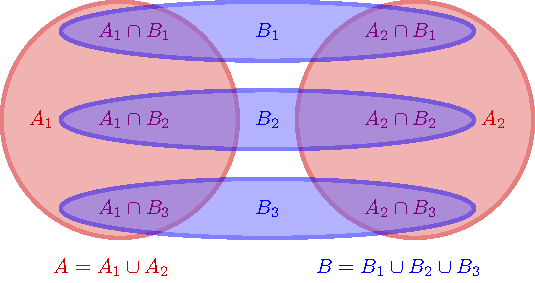
\includegraphics{fig-1-5}
	\caption{Подання множин $A$ і $B$.}
	\label{fig-1-5}
\end{figure}
\item \label{th-1-3-3}
Маємо (див. рис. \ref{fig-1-5}) 
\begin{align}
\label{th-1-3.1}
A\setminus B&= \bigcup_{k=1}^n (A_k\setminus B),
\\
\label{th-1-3.2} 
A_k\setminus B&= A_k\setminus \left(\bigcup_{i=1}^j B_i\right)
= \bigcap_{i=1}^j (A_k\setminus B_i),\quad k=\overline{1,n}.
\end{align}
Для будь-яких $k=\overline{1,n}$ і $i=\overline{1,j}$ маємо $A_k\in \PP$ і $B_i\in\PP$, тому
$$
A_k\setminus B_i=\bigcup_{r=1}^{s} C_r^{ki},
$$
де $\PP\supset\{C_r^{ki}\}_{r=1}^s$ є неперетинними. Отже, $A_k\setminus B_i\in\mathcal L$, $k=\overline{1,n}$, $i=\overline{1,j}$. Ураховуючи \eqref{th-1-3.2}, згідно з кроком \ref{th-1-3-2} маємо 
$A_k\setminus B\in\mathcal L$, $k=\overline{1,n}$.  Оскільки $\{A_k\setminus B\}_{k=1}^n$  є неперетинними, беручи до уваги крок \ref{th-1-3-1} і \eqref{th-1-3.1}, одержуємо $A\setminus B\in\mathcal L$.
\item \label{th-1-3-4}
Маємо
$$
A\cup B=(A\setminus B)\cup(A\cap B)\cup(B\setminus A),
$$
де $A\setminus B$, $A\cap B$, $B\setminus A$ є неперетинними. Згідно з кроком \ref{th-1-3-2}  $A\cap B\in\mathcal L$,  а згідно з кроком \ref{th-1-3-3} $A\setminus B\in\mathcal L$ і $B\setminus A\in\mathcal L$. Тому, беручи до уваги крок \ref{th-1-3-1}, одержуємо $A\cup B\in\mathcal L$. 
\begin{figure}[!h]
	\centering
	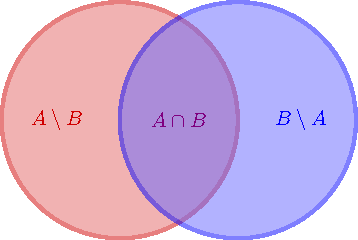
\includegraphics{fig-1-6}
	\caption{Подання об'єднання множин $A$ і $B$.}
	\label{fig-1-6}
\end{figure}
\end{enumerate}

Таким чином, $\mathcal L$ є кільцем.    Оскільки $\PP\subset\mathcal L$ за побудовою,    скориставшись означенням кільця, породженого заданим класом множин (див. означення \ref{def-1-7}), одержуємо $\mathcal L\supset k(\PP)$.  Крім того, ми вже довели, що $\mathcal L\subset k(\PP)$. Отже, $\mathcal L= k(\PP)$, тобто \eqref{1.5}  виконано. Теорему доведено.
\end{proof}

\begin{example}
\label{ex-1-10}
Згідно з цією теоремою для півкільця $\PP_1$ з прикладу  \ref{ex-1-4} маємо
$$
k(\PP_1)=\left\{\bigcup_{k=1}^n (a_k,b_k] \midd n\in\N \land \R\supset\{(a_k,b_k]\}_{k=1}^n \ \text{є неперетинними} \right\}.
$$
\end{example}

\begin{example}
\label{ex-1-10-a}
Згідно з цією теоремою  для півкільця $\PP_d$ з прикладу  \ref{ex-1-5} маємо
\begin{align*}
k(\PP_d)&=\left\{\bigcup_{k=1}^n \left(\bigtimes_{m=1}^d\left(a_m^k,b_m^k\right]\right) \midd
\right.
\\
&\hspace{25mm}\left.
 n\in\N\ \land\ \R^d\supset\left\{ \bigtimes_{m=1}^d\left(a_m^k,b_m^k\right]\right\}_{k=1}^n \ \text{є неперетинними} \right\}.
\end{align*}
\end{example}

\section{Дві теореми про породжені класи}

\begin{definition}
	\label{intersec}
	Нехай $B\subset X$ і $\HH\subset 2^X$. Позначимо
	$$
	\HH\cap B=\{a\cap B \mid A\in\HH\}.
	$$
\end{definition}

Розглянемо теорему про перетин $\sigma$-кільця.

\begin{theorem}
	\label{th-1-4}
	Нехай $B\subset X$ і $\HH\subset 2^X$. Тоді
	$$
	\sigma k(\HH\cap B)=\sigma k(\HH)\cap B.
	$$
\end{theorem}

\begin{proof}
	Доведення цієї рівності розіб'ємо на дві частини: $\sigma k(\HH\cap B)\subset\sigma k(\HH)\cap B$ і $\sigma k(\HH\cap B)\supset\sigma k(\HH)\cap B$.
	
	Нехай $\{A_n\}_{n=1}^\infty\subset \sigma k(\HH)$. Маємо  $\displaystyle \bigcup_{n=1}^\infty A_n\in \sigma k(\HH)$, $A_1\setminus A_1\in \sigma k(\HH)$, $\{A_n\cap B\}_{n=1}^\infty\subset \sigma k(\HH)\cap B$ і (див. рис. \ref{fig-1-7})
	\begin{align*}
	\bigcup_{n=1}^\infty (A_n\cap B)& = \left(\bigcup_{n=1}^\infty A_n\right)\cap B \in \sigma k(\HH)\cap B,
	\\
	(A_1\cap B)\setminus (A_2\cap B)&= (A_1\setminus A_2) \cap B\in \sigma k(\HH)\cap B.
	\end{align*}
	\begin{figure}[!h]
		\centering
		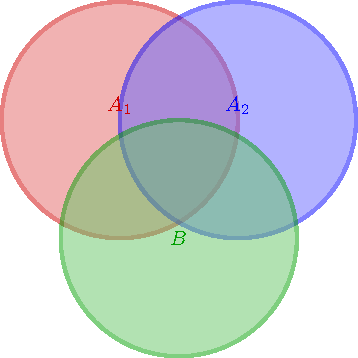
\includegraphics{fig-1-7}
		\caption{Подання об'єднання множин $A$ і $B$.}
		\label{fig-1-7}
	\end{figure}
	Тому $\sigma k(\HH)\cap B$ є $\sigma$-кільцем. Оскільки $\HH\subset \sigma k(\HH)$, маємо $\HH\cap B \subset \sigma k(\HH)\cap B$. Отже, $\sigma k(\HH\cap B)\subset\sigma k(\HH)\cap B$ тому, що $\sigma k(\HH)\cap B$ є $\sigma$-кільцем.
	
	Далі розглянемо клас множин
	\begin{equation}
	\label{1.7}
	\mathcal L= \big\{A\cup(C\setminus B) \mid A\in \sigma k(\HH\cap B) \land C\in \sigma k(\HH)\big\}.
	\end{equation}
	
	Перевіримо, що $\mathcal L$ є $\sigma$-кільцем. Нехай $\{A_n\}_{n=1}^\infty\subset \sigma k(\HH\cap B)$, $C\in \sigma k(\HH)$. Тоді $\displaystyle \bigcup_{n=1}^\infty A_n\in \sigma k(\HH\cap B)$, $A_1\setminus A_2\in \sigma k(\HH\cap B)$, $\{A_n\cup(C\setminus B)\}_{n=1}^\infty\subset \mathcal L$ і
	\begin{align*}
	\bigcup_{n=1}^\infty (A_n\cup(C\setminus B))& = \left(\bigcup_{n=1}^\infty A_n\right)\cup(C\setminus B) \in \mathcal L,
	\\
	(A_1\cup(C\setminus B))\setminus (A_2\cup(C\setminus B))&= (A_1\setminus A_2) \cup(C\setminus B)\in \mathcal L
	\end{align*}
	(див. рис. \ref{fig-1-7}, де в якості множини $B$  розглядається $C\setminus B$).
	Тому $\mathcal L$ є $\sigma$-кільцем. Для $D\in\HH$ маємо $D\in \sigma k(\HH)$ і
	$$
	D=(D\cap B)\cup (D\setminus B).
	$$
	Оскільки $D\cap B\subset \HH\cap B\subset \sigma k(\HH\cap B)$, маємо $D\in\mathcal L$. Отже, $\HH\subset \mathcal L$. З того, що $\mathcal L$ є $\sigma$-кільцем випливає $\sigma k(\HH)\subset \mathcal L$. Тому $\sigma k(\HH)\cap B\subset \mathcal L\cap B=\sigma k(\HH\cap B)$ в останній рівності враховано співвідношення \eqref{1.7}. Теорему доведено. 
\end{proof}

Розглянемо теорему про рівність монотонного класу і $\sigma$-кільця, породженого кільцем.

\begin{theorem}
	\label{th-1-5}
	Нехай $\K\subset 2^X$ є кільцем. Тоді $m(\K)=\sigma k(\K)$.
\end{theorem}

\begin{proof}  
	Оскільки клас $\sigma k(\K)$ є $\sigma$-кільцем, цей клас є замкненим відносно взяття нескінченного об'єднання (за означенням \ref{def-1-4}) і нескінченного перетину (за теоремою \ref{st-pr-sring}) тому він є монотонним класом. Ураховуючи те, що  $\K\subset \sigma k(\K)$, одержуємо $m(\K)\subset \sigma k(\K)$.
	
	Доведемо тепер протилежне включення. Спочатку доведемо, що $m(\K)$ є кільцем.
	
	Зафіксуємо довільну множину $D\in m(\K)$ і розглянемо клас множин
	$$
	\LL(D)=\big\{C\in X\mid D\cup C\in m(\K) \land D\setminus C\in m(\K) \land C\setminus D\in m(\K) \big\}.
	$$
	Перевіримо, що $\LL(D)$ є монотонним класом. Нехай $\{C_n\}_{n=1}^\infty\uparrow\subset \LL(D)$ і
	$$
	C=\lim_{n\to\infty} C_n=\bigcup_{n=1}^\infty C_n.
	$$ 
	Маємо $\{D\cup C_n\}_{n=1}^\infty\uparrow\subset m(\K)$, $\{D\setminus C_n\}_{n=1}^\infty\downarrow\subset m(\K)$, $\{ C_n\setminus D\}_{n=1}^\infty\uparrow\subset m(\K)$. Оскільки $m(\K)$ є монотонним класом, маємо
	\begin{align*}
	D\cup C&=D\cup \left(\bigcup_{n=1}^\infty C_n\right) = \bigcup_{n=1}^\infty (D\cup C_n)\in m(\K),
	\\
	D\setminus C&=D\setminus \left(\bigcup_{n=1}^\infty C_n \right)= \bigcap_{n=1}^\infty (D\setminus C_n)\in m(\K),
	\\
	C\setminus D&=\left(\bigcup_{n=1}^\infty C_n\right) \setminus D = \bigcup_{n=1}^\infty (C_n\setminus D)\in m(\K),
	\end{align*}
	тобто $C\in\LL(D)$. Цілком аналогічно перевіряємо, що для $\{C_n\}_{n=1}^\infty\downarrow\subset \LL(D)$ і
	$$
	C=\lim_{n\to\infty} C_n=\bigcap_{n=1}^\infty C_n\in\LL(D).
	$$ 
	Отже, $\LL(D)$ є монотонним класом.
	
	Якщо $E\in\K$ і $F\in\K$, то
	$$
	E\cup F\in\K\subset m(\K),\quad E\setminus F\in\K\subset m(\K),\quad F\setminus E\in\K\subset m(\K)
	$$
	тому, що $\K$ є кільцем. Отже, $F\in\LL(E)$ і $\K\subset\LL(E)$ оскільки $F\in\K$ вибрано довільним. З того, що $\LL(E)$ є монотонним класом випливає $m(\K)\subset\LL(E)$ для $E\in\K$.
	
	Отже, для будь-якої множини $B\in m(\K)$ маємо $B\in\LL(E)$, тому 
	$$
	E\cup B\in m(\K),\quad E\setminus B\in m(\K),\quad B\setminus E\in m(\K).
	$$
	Це означає, що $E\in\LL(B)$. Отже, $\K\subset\LL(B)$ оскільки $E\in\K$ вибрано довільним. З того, що $\LL(B)$ є монотонним класом випливає $m(\K)\subset\LL(B)$ тепер вже для $B\in m(\K)$.
	
	Нехай $A\in m(\K)$ і $B\in m(\K)$. Тоді $A\in\LL(B)$ і
	$$
	A\cup B\in m(\K),\quad A\setminus B\in m(\K),\quad B\setminus A\in m(\K).
	$$
	Отже, $m(\K)$ є кільцем.
	Оскільки $m(\K)$ є монотонним класом і кільцем одночасно, то за теоремою \ref{th-1-2} про зв'язок між кільцем і монотонним класом $m(\K)$ є $\sigma$-кільцем. З того, що $\K\subset m(\K)$ випливає $\sigma k(\K)\subset m(\K)$. Оскільки протилежне включення також є вірним, то $\sigma k(\K)= m(\K)$. Теорему доведено.
\end{proof}

\section{Борельові множини}

Клас борельових множин є одним з найважливіших прикладів породжених $\sigma$-алгебр. Нехай на множині $X$ задано метрику $\rho$. Розглянемо метричний простір $(X,\rho)$ і позначимо через $\mathscr G_X$ клас усіх відкритих підмножин $X$.

\begin{definition}
	\label{def-1-8}
	Борельовою $\sigma$-алгеброю в $Y$ (позначається $\BB(X)$) називається $\sigma a\big(\mathscr G_X\big)$. Множини з $\BB(X)$ називаються борельовими.
\end{definition}

\begin{example}
	\label{ex-b-1}
	Будь-яка відкрита множина $U\subset X$ є борельовою тому, що $U\in\mathscr G_X\subset \sigma a\big(\mathscr G_X\big)=\BB\big(X\big)$.
\end{example}

\begin{example}
	\label{ex-b-2}
	Будь-яка замкнена множина $F$ є болельовою.  Дійсно, $X\setminus F$ є відкритою і $X\setminus F\in\mathscr G_X\subset \BB(X)$. Оскільки $\BB(X)$ є $\sigma$-алгеброю, маємо $F=X\setminus(X\setminus F)$.
\end{example}

\begin{example}
	\label{ex-b-3}
	Одноточкова множина є борельовою, оскільки вона є замкненою. 
\end{example}

\begin{example}
	\label{ex-b-4}
	Усі скінченні, зліченні множини та їх доповнення є борельовими, оскільки їх можна подати увигляді скінченного або зліченного об'єднання одноточкових множин та їх доповнення, а $\sigma$-алгебра є замкненою відносно цих операцій. 
\end{example}

Розглянемо теорему про подання борельової $\sigma$-алгебри підмножин $\R^d$.

\begin{theorem}
	\label{th-1-6}
	Для півкільця підмножин $\R^d$
	$$
	\PP_d=\left\{\bigtimes_{k=1}^d (a_k,b_k]\midd \forall k=\overline{1,d}\ -\infty< a_k\leq b_k< +\infty\right\}
	$$
	маємо
	$$
	\sigma k(\PP_d)=\sigma a(\PP_d)=\BB(\R^d).
	$$
\end{theorem}

\begin{proof}
	Оскільки
	$$
	\R^d=\bigcup_{n=1}^\infty (-n,n]^d,
	$$
	маємо $\R^d\in \sigma k(\PP_d)$, отже, 
	\begin{equation}
	\label{1.8}
	\sigma k(\PP_d)=\sigma a(\PP_d).
	\end{equation}

Нехай
$$
A=\bigtimes_{k=1}^d (a_k,b_k]\in\PP_d, \quad A_n=\bigtimes_{k=1}^d \left(a_k,b_k+\frac1n\right),\quad n\in\N.
$$
Тоді $A_n$ є відкритою множиною тому
$A_n\in\BB(\R^d)$, $n\in\N$, і $\displaystyle A=\bigcap_{n=1}^\infty A_n$. Отже, $A\in\BB(\R^d)$ тому $\PP_d\subset\BB(\R^d)$. Звідси випливає 
\begin{equation}
\label{1.9}
\sigma a(\PP_d)\subset\BB(\R^d).
\end{equation}


Залишилося довести протилежне включення. Нехай $U$ є відкритою множиною в $\R^d$. Тоді
\begin{equation}
\label{1.10}
U=\bigcup_{(p,q)\in\mathcal Q} \bigtimes_{k=1}^d (p_k,q_k], 
\end{equation}
де 
\begin{align*}
\mathcal Q&= \left\{(u,v)=\left(\begin{pmatrix}u_1\\ \vdots\\ u_d \end{pmatrix}, \begin{pmatrix}v_1\\ \vdots\\ v_d \end{pmatrix}\right)\in\overline{\Q}{}^d\times \overline{\Q}{}^d \midd 
\right.
\\
&\kern20ex\left. \vphantom{\begin{pmatrix}u_1\\ \vdots\\ u_d \end{pmatrix}}
\bigtimes\limits_{k=1}^d (u_k,v_k]\subset U \land \big(\forall k=\overline{1,d}\   u_k<v_k\big)\right\}.
\end{align*} 
Зрозуміло, що права частина \eqref{1.10} є об'єднанням підмножин $U$, тому сама є підмножиною $U$. З іншого боку, кожна точка відкритої множини $U$ має окіл вигляду  $\bigtimes\limits_{k=1}^d (p_k,q_k]$, $p_k\in\Q$, $q_k\in\Q$, $k=\overline{1,d}$, який міститься в $U$. Тому $U$ міститься об'єднанні, що стоїть у правій частині \eqref{1.10}. Таким чином рівність \eqref{1.10} має місце.

Об'єднання в правій частині \eqref{1.10} є зліченним, тому $U\in \sigma a (\PP_d)$. Отже,  $\mathscr G_\R\subset \sigma a (\PP_d)$, тому 
\begin{equation}
\label{1.11}
\BB\big(\R^d\big)=\sigma a \big(\mathscr G_\R\big)\subset \sigma a \big(\PP_d\big).
\end{equation}
Зі співвідношень  \eqref{1.8}, \eqref{1.9} і \eqref{1.11} випливає твердження теореми.	
\end{proof}

